\chapter{GRASP}

\section{Modificaciones a la heuristica constructiva}
Para poder aplicar nuestra heuristica constructiva a un procedimiento GRASP, fue necesario introducir algun factor de aleatoriedad a la misma.

Nosotros consideramos dos formas de hacerlo:
\begin{enumerate}
\item Modificar el criterio de elecci�n del nodo candidato en la inserci�n:
Se considera un valor $\alpha \in [0,1]$, de modo que en cada paso no se selecciona el de grado m�ximo, sino que se selecciona un v tal que $d(v) \geq \alpha*d_{max}$. Si $\alpha = 1$, la elecci�n no es aleatoria, en cambio si $\alpha = 0$, se escoge un candidato totalmente al azar. En general, en (0,1), un $\alpha$ mas grande implica una lista restringida de candidatos mas peque�a.

\item Modificar el criterio de elecci�n de la posici�n:
Nuestra heuristica constructiva frente a un ``empate'' de posiciones, es decir, para un nodo dado, hay dos o mas posiciones que generan la misma cantidad de cruces, lo que hace es quedarse con la primera visitada. 

\begin{figure}[H]
\centering
\setcounter{subfigure}{0}
\subfigure[]{
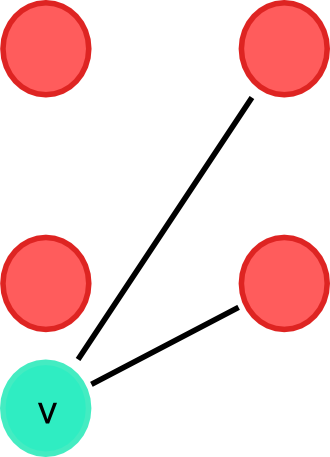
\includegraphics[scale=0.15]{./figuras/grasp/empate1.png}}
\setcounter{subfigure}{1}
\subfigure[]{
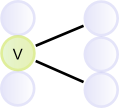
\includegraphics[scale=0.15]{./figuras/grasp/empate2.png}}
\subfigure[]{
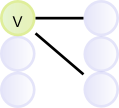
\includegraphics[scale=0.15]{./figuras/grasp/empate3.png}}
\caption{Empate entre posiciones: cualquiera de las 3 posiciones es a priori tan buena como las otras}
\end{figure}

Entonces podemos modificar esto, para que si hay empate eliga alguna de todas estas posiciones al azar.

\end{enumerate}
Posteriormente realizaremos, experiencias con el fin de determinar si estas modificaciones son utilies, y ademas con el fin de determinar que valor de $\alpha$ debe usarse.

\section{Determinaci�n de los parametros}

\subsection{Criterios de parada}
% deberian ir juntos
\subsection{Tama�o de la lista de candidatos}

\section{Pseudocodigo}

\section{Calculo de complejidad}

\section{Analisis experimental}


\section{Discusi�n}
